\documentclass[journal,12pt,twocolumn]{IEEEtran}

\usepackage{setspace}
\usepackage{gensymb}

\singlespacing
\usepackage{pstricks}
\usepackage[cmex10]{amsmath}
%\usepackage{amsthm}
%\interdisplaylinepenalty=2500
%\savesymbol{iint}
%\usepackage{txfonts}
%\restoresymbol{TXF}{iint}
%\usepackage{wasysym}
\usepackage{amsthm}
%\usepackage{iithtlc}
\usepackage{mathrsfs}
\usepackage{txfonts}
\usepackage{stfloats}
\usepackage{bm}
\usepackage{cite}
\usepackage{cases}
\usepackage{subfig}
%\usepackage{xtab}
\usepackage{longtable}
\usepackage{multirow}
%\usepackage{algorithm}
%\usepackage{algpseudocode}
\usepackage{enumitem}
\usepackage{mathtools}
\usepackage{caption}
\usepackage{steinmetz}
\usepackage{tikz}
%\usepackage{circuitikz}
\usepackage{verbatim}
\usepackage{tfrupee}
\usepackage[breaklinks=true]{hyperref}
%\usepackage{stmaryrd}
\usepackage{tkz-euclide} % loads  TikZ and tkz-base
%\usetkzobj{all}
\usetikzlibrary{calc,math}
\usepackage{listings}
\usepackage{color}                                            %%
\usepackage{array}                                            %%
\usepackage{longtable}                                        %%
\usepackage{calc}                                             %%
\usepackage{multirow}                                         %%
\usepackage{hhline}                                           %%
\usepackage{ifthen}                                           %%
%optionally (for landscape tables embedded in another document): %%
\usepackage{lscape}     
%\usepackage{multicol}
\usepackage{chngcntr}
%\usepackage{enumerate}
%\usepackage{wasysym}
%\newcounter{MYtempeqncnt}
\DeclareMathOperator*{\Res}{Res}
%\renewcommand{\baselinestretch}{2}
\renewcommand\thesection{\arabic{section}}
\renewcommand\thesubsection{\thesection.\arabic{subsection}}
\renewcommand\thesubsubsection{\thesubsection.\arabic{subsubsection}}

\renewcommand\thesectiondis{\arabic{section}}
\renewcommand\thesubsectiondis{\thesectiondis.\arabic{subsection}}
\renewcommand\thesubsubsectiondis{\thesubsectiondis.\arabic{subsubsection}}

% correct bad hyphenation here
\hyphenation{op-tical net-works semi-conduc-tor}
\def\inputGnumericTable{}                                 %%

\lstset{
	%language=C,
	frame=single, 
	breaklines=true,
	columns=fullflexible
}
\usepackage{amssymb}
\usepackage{stackengine}
\usepackage{scalerel}
\usepackage{graphicx}
\newlength\lthk
\setlength\lthk{.1ex}
\def\bline{\rule{2ex}{\lthk}}
\def\slash{\rotatebox{60}{\bline}}
\def\parallelogram{\stackMath\scalerel*{%
		\def\stackalignment{l}{\stackunder[-.5\lthk]{%
				\def\stackalignment{r}\stackon[-.5\lthk]{\slash\rule{.866ex}{0ex}\slash}{\bline}}%
			{\bline}}}{\square}%
}

\begin{document}
	%
	
	
	\newtheorem{theorem}{Theorem}[section]
	\newtheorem{problem}{Problem}
	\newtheorem{proposition}{Proposition}[section]
	\newtheorem{lemma}{Lemma}[section]
	\newtheorem{corollary}[theorem]{Corollary}
	\newtheorem{example}{Example}[section]
	\newtheorem{definition}[problem]{Definition}
	
	\newcommand{\BEQA}{\begin{eqnarray}}
		\newcommand{\EEQA}{\end{eqnarray}}
	\newcommand{\define}{\stackrel{\triangle}{=}}
	\bibliographystyle{IEEEtran}
	%\bibliographystyle{ieeetr}
	\providecommand{\mbf}{\mathbf}
	\providecommand{\pr}[1]{\ensuremath{\Pr\left(#1\right)}}
	\providecommand{\qfunc}[1]{\ensuremath{Q\left(#1\right)}}
	\providecommand{\sbrak}[1]{\ensuremath{{}\left[#1\right]}}
	\providecommand{\lsbrak}[1]{\ensuremath{{}\left[#1\right.}}
	\providecommand{\rsbrak}[1]{\ensuremath{{}\left.#1\right]}}
	\providecommand{\brak}[1]{\ensuremath{\left(#1\right)}}
	\providecommand{\lbrak}[1]{\ensuremath{\left(#1\right.}}
	\providecommand{\rbrak}[1]{\ensuremath{\left.#1\right)}}
	\providecommand{\cbrak}[1]{\ensuremath{\left\{#1\right\}}}
	\providecommand{\lcbrak}[1]{\ensuremath{\left\{#1\right.}}
	\providecommand{\rcbrak}[1]{\ensuremath{\left.#1\right\}}}
	\theoremstyle{remark}
	\newtheorem{rem}{Remark}
	\newcommand{\sgn}{\mathop{\mathrm{sgn}}}
	\providecommand{\abs}[1]{\left\vert#1\right\vert}
	\providecommand{\res}[1]{\Res\displaylimits_{#1}} 
	\providecommand{\norm}[1]{\left\lVert#1\right\rVert}
	%\providecommand{\norm}[1]{\lVert#1\rVert}
	\providecommand{\mtx}[1]{\mathbf{#1}}
	\providecommand{\mean}[1]{E\left[ #1 \right]}
	\providecommand{\fourier}{\overset{\mathcal{F}}{ \rightleftharpoons}}
	%\providecommand{\hilbert}{\overset{\mathcal{H}}{ \rightleftharpoons}}
	\providecommand{\system}{\overset{\mathcal{H}}{ \longleftrightarrow}}
	%\newcommand{\solution}[2]{\textbf{Solution:}{#1}}
	\newcommand{\solution}{\noindent \textbf{Solution: }}
	\newcommand{\cosec}{\,\text{cosec}\,}
	\providecommand{\dec}[2]{\ensuremath{\overset{#1}{\underset{#2}{\gtrless}}}}
	\newcommand{\myvec}[1]{\ensuremath{\begin{pmatrix}#1\end{pmatrix}}}
	\newcommand{\mydet}[1]{\ensuremath{\begin{vmatrix}#1\end{vmatrix}}}
	%\numberwithin{equation}{section}
	\numberwithin{equation}{subsection}
	%\numberwithin{problem}{section}
	%\numberwithin{definition}{section}
	\makeatletter
	\@addtoreset{figure}{problem}
	\makeatother
	\let\StandardTheFigure\thefigure
	\let\vec\mathbf
	%\renewcommand{\thefigure}{\theproblem.\arabic{figure}}
	\renewcommand{\thefigure}{\theproblem}
	%\setlist[enumerate,1]{before=\renewcommand\theequation{\theenumi.\arabic{equation}}
	%\counterwithin{equation}{enumi}
	%\renewcommand{\theequation}{\arabic{subsection}.\arabic{equation}}
	\def\putbox#1#2#3{\makebox[0in][l]{\makebox[#1][l]{}\raisebox{\baselineskip}[0in][0in]{\raisebox{#2}[0in][0in]{#3}}}}
	\def\rightbox#1{\makebox[0in][r]{#1}}
	\def\centbox#1{\makebox[0in]{#1}}
	\def\topbox#1{\raisebox{-\baselineskip}[0in][0in]{#1}}
	\def\midbox#1{\raisebox{-0.5\baselineskip}[0in][0in]{#1}}
	\vspace{3cm}
	\title{Assignment-5}
	\author{Pooja H \\ AI20MTECH14003}
	\maketitle
	\newpage
	\bigskip
	\renewcommand{\thefigure}{\theenumi}
	\renewcommand{\thetable}{\theenumi}
\begin{abstract}
	In this work, we estimate the area of triangle with vector representation.
\end{abstract}
%Download all python codes from 
%\begin{lstlisting}
%	https://github.com/poojah15/EE5609_AI20MTECH14003/tree/master/Assignment_5
%\end{lstlisting}
Download all latex-tikz codes from 
\begin{lstlisting}
	https://github.com/poojah15/EE5609_AI20MTECH14003/tree/master/Assignment_5
\end{lstlisting}
\section{Problem Statement}
Prove that the triangles on the same base (or equal bases) and between the same parallels are equal in area.
\section{Solution}
Let ABC and ABD are the given triangles with the same base AB and between the same parallel lines AB and CD.
\renewcommand{\thefigure}{1}
\begin{figure}[!ht]
\centering
\resizebox{\columnwidth}{!}{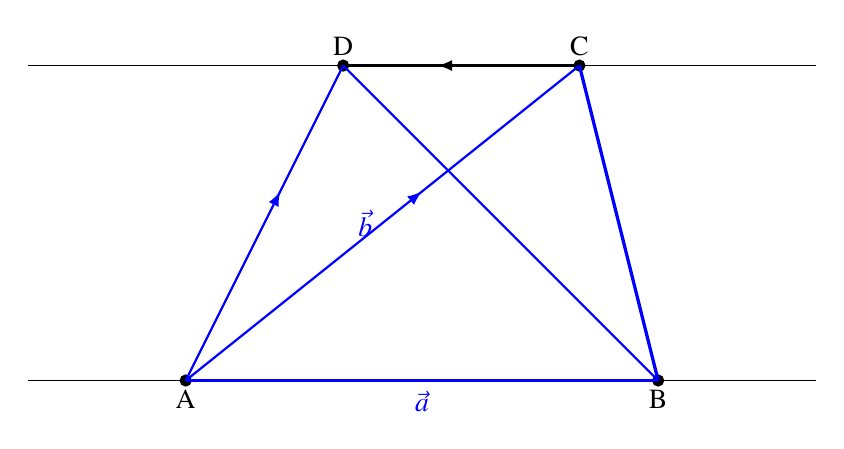
\begin{tikzpicture}[decoration = {markings, mark = at position 0.6 with {\arrow{latex}}
		}]
		\draw (-2,0) -- (8,0);
		\draw (-2,4) -- (8,4);
    	\filldraw[black] (0,0) circle (2pt) node[anchor=north] {A};
		\filldraw[black] (6,0) circle (2pt) node[anchor=north] {B};
		\filldraw[black] (2,4) circle (2pt) node[anchor=south] {D};
		\filldraw[black] (5,4) circle (2pt) node[anchor=south] {C};
	    \draw[blue, thick] (0, 0) -- (6, 0) node[midway, below] {$\vec{a}$};
	    \draw[postaction = decorate, blue, thick] (0, 0) -- (2, 4);
	    \draw[postaction = decorate, black, thick] (5, 4) -- (2, 4);
	     \draw[postaction = decorate,blue, thick] (0, 0) -- (5, 4) node[midway, left]{$\vec{b}$};
	    \draw[blue, thick] (6,0) -- (2, 4);
	   	 \draw[blue, very thick] (5, 4) -- (6,0);
\end{tikzpicture}
}
\caption{Triangles on same base} 
\end{figure}\\
Let AB = $\vec{a}$ and AC = $\vec{b}$. Also the lines AB and CD are parallel, which implies that CD = k $\times$ AB.
Here, the area of $\triangle$ ABC is given by
\begin{align} 
	  Area(\triangle ABC) = \frac{1}{2}(\vec{a} \times \vec{b})\label{eq:eq1}
\end{align}
And, the area of $\triangle$ ABD is given by
\begin{align}
	\frac{1}{2}(AB \times AD) &= (\vec{a} \times (AC + CD))\\
	&= \frac{1}{2}(\vec{a} \times  (\vec{b} + k\vec{a}))\\
	&= \frac{1}{2}(\vec{a} \times  \vec{b}) + (\vec{a} \times  k\vec{a})\\
	&= \frac{1}{2}(\vec{a} \times  \vec{b}) + k (\vec{a} \times  \vec{a})\\
	Area(\triangle ABD)&= \frac{1}{2}(\vec{a} \times  \vec{b})  \quad [\because \vec{a} \times  \vec{a} =0] \label{eq:eq2}
\end{align}
From \eqref{eq:eq1} and \eqref{eq:eq2}, we can infer that the area of two triangles are one and the same.
Hence, it is proved that the triangles on the same base and between the same parallels are equal in area.

\end{document}